%!TEX root = MemoireZelliges.tex

\chapter{Problématique}
%======================================================================

\renewcommand{\putstuffinpic}{%
  \put(100,-140){%
    \makebox(0,0){%
      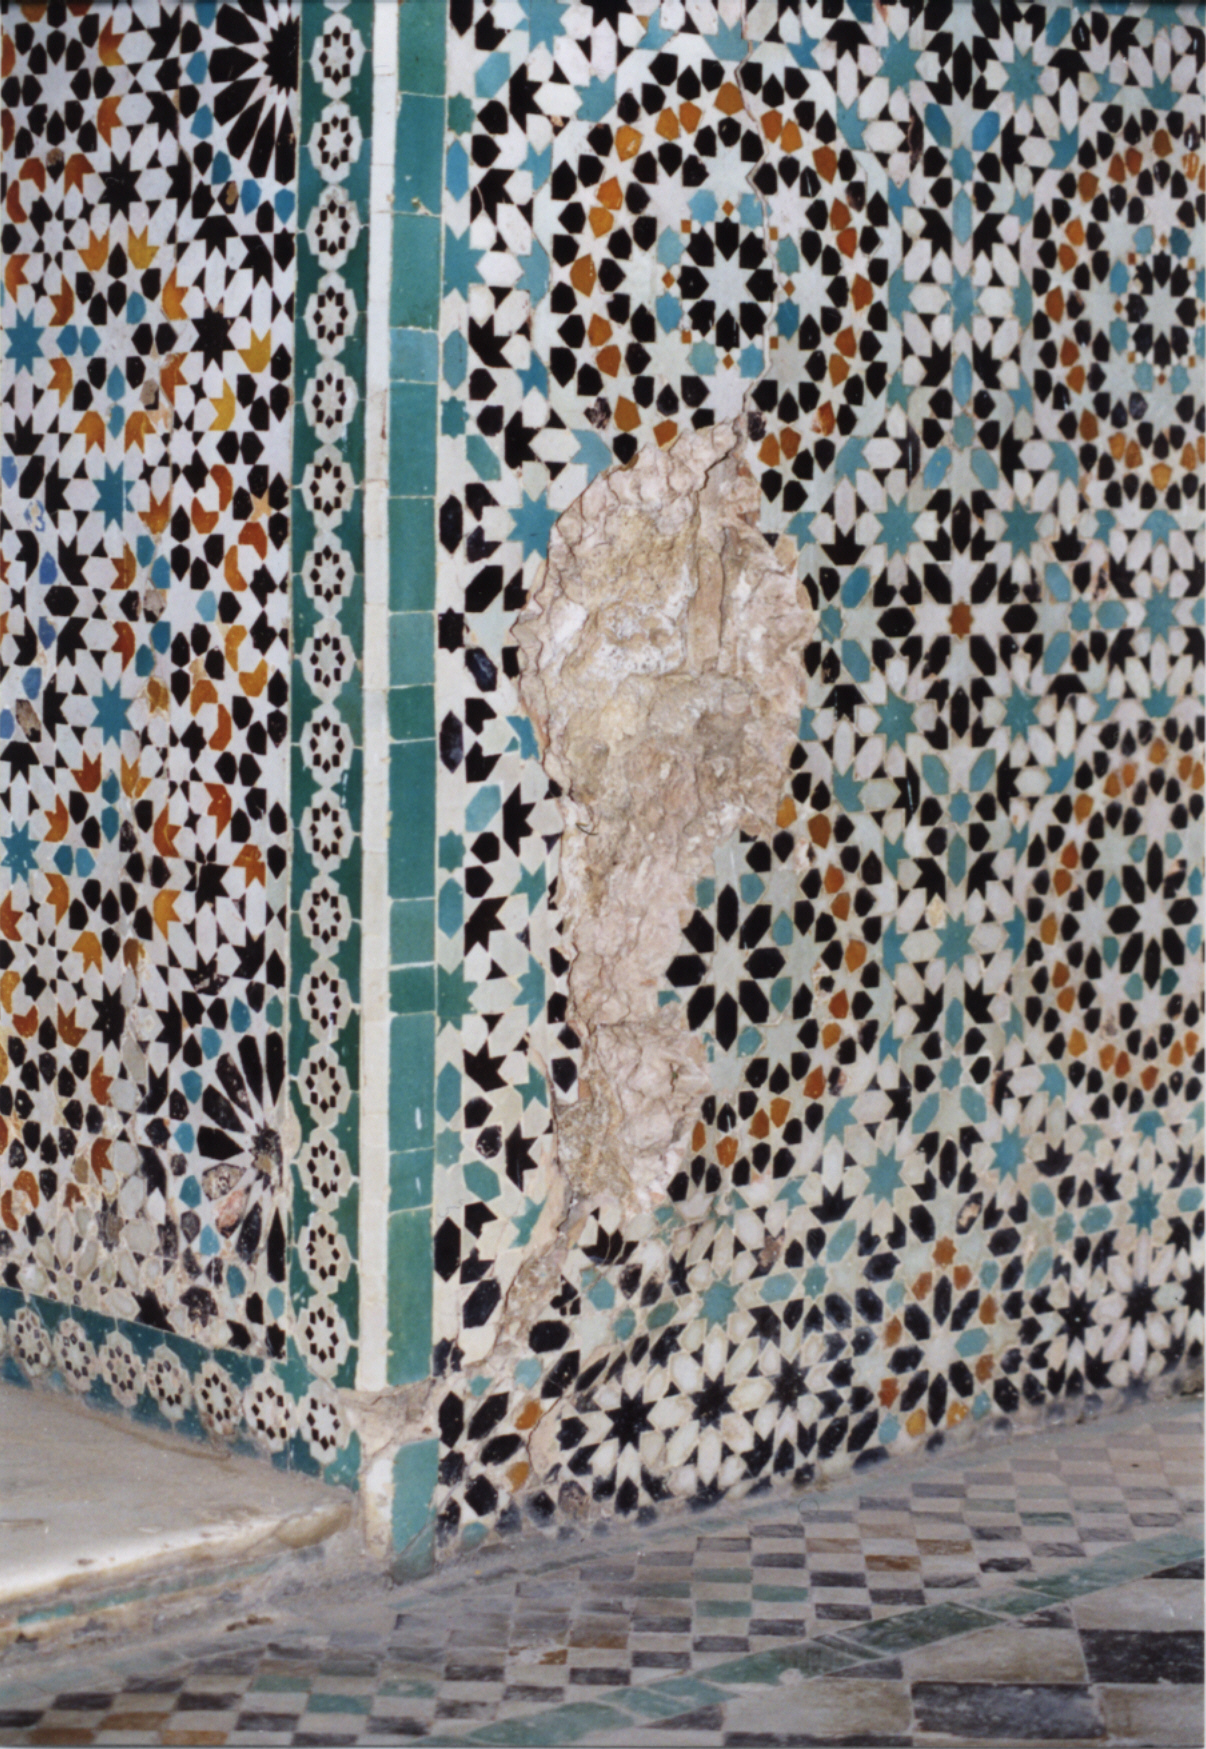
\includegraphics[width=0.45\textwidth]{alteration_1}%
      \quad%
      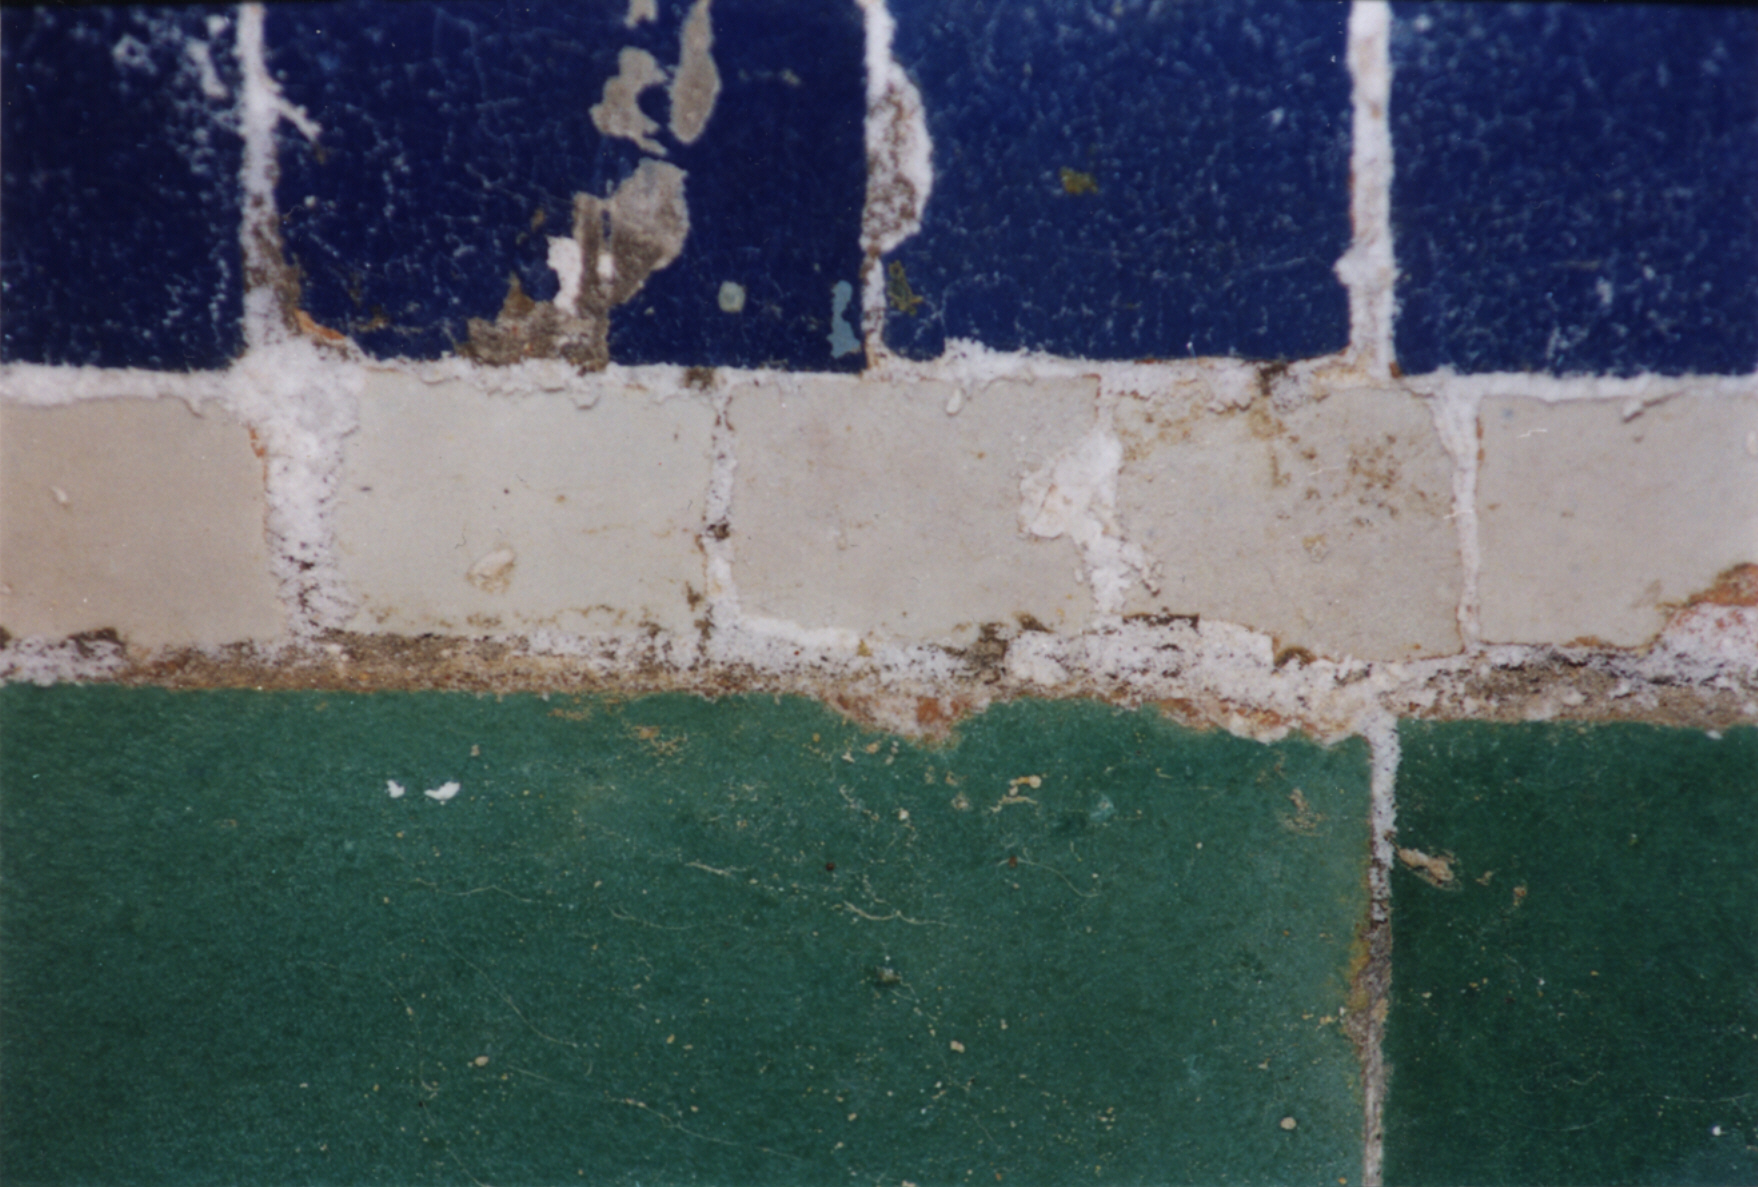
\includegraphics[width=0.45\textwidth]{alteration_2}%
      % \captionof{figure}{Différents types d'altération : à gauche, on note 
      %          un décollement d'une partie du panneau décoré de 
      %          zelliges ;
      %          à droite, des efflorescences salines sont visibles 
      %          entre les pièces de céramique (clichés :~Schv{\oe}rer, 
      %          1999).}
      % \label{fig:alteration}
    }%
  }%
}
\newcommand{\mycut}{%
  0.5\textwidth,
  0.5\textwidth,
  0.5\textwidth,
  0.5\textwidth,
  0.5\textwidth,
  0.5\textwidth,
  0.5\textwidth,
  0.5\textwidth,
  0.5\textwidth,
  0.5\textwidth,
  0.5\textwidth,
  0.5\textwidth,
  0.5\textwidth,
  0.5\textwidth,
  0.5\textwidth%
}%
\opencutleft%<
L'architecture musulmane, et donc celle du Maroc, est intimement 
liée à la religion. Les premiers conquérants nomades n'étaient pas 
des bâtisseurs. Cependant la liturgie de l'Islam nécessite une 
architecture pour rassembler les fidèles lors de la prière commune du 
vendredi. À l'origine très rudimentaire, cette architecture va peu à 
peu s'enrichir au contact de celles, prestigieuses, des civilisations 
conquises. La \emph{mosquée du vendredi} (\emph{Masj'id-el-Djami}) 
qui réunit l'assemblée (\emph{Ouma}) n'est pas seulement un lieu de 
prière, c'est également là que l'on discute des affaires courantes. 
On peut donc dire qu'elle a un rôle particulièrement important dans 
la vie de la communauté.

C'est dans l'architecture, d'abord religieuse, que l'art islamique a 
trouvé l'un de ses lieux d'application privilégiés, l'autre étant le 
livre. Avec le développement des cités, les principes décoratifs 
inventés pour les mosquées ont été transposés dans l'architecture 
civile.

Le Maroc a développé une forme d'art tout à fait particulière : 
l'art des zelliges. Il s'agit d'un revêtement de mosaïque de 
céramique glaçurée, décorant à la fois les murs et les sols.
L'art des zelliges et les bâtiments qu'il décore font partie 
intégrante de la vie et du patrimoine culturel du Maroc. 
Malheureusement, ces témoignages du passé sont aujourd'hui 
victimes des ravages du temps : des panneaux entiers de zelliges 
se détachent, les glaçures sont altérées, on note également la 
présence d'efflorescences salines entre les pièces de céramique
(\fref{fig:alteration}).

\bigskip

\begin{shapedcutout}{3}{15}{\mycut}
Les architectes marocains souhaitent restaurer ces monuments et 
leurs décors de zelliges, en recréant les pièces manquantes selon 
les techniques anciennes, et dans la mesure du possible, mettre en 
{\oe}uvre une politique de conservation préventive. Mais ces 
techniques ne sont pas connues et les artisans actuels se sont 
adaptés aux matériaux modernes et colorants de synthèse.
La problématique de cette étude, portant sur les problèmes de 
préservation des céramiques glaçurées architecturales, s'articule 
donc autour de deux thèmes, dans le but de fournir aux architectes 
les données physico-chimiques nécessaires à leurs travaux : d'une 
part la recherche des techniques de fabrication anciennes, d'autre 
part l'évaluation et la caractérisation des phénomènes d'altération 
rencontrés dans ce type de matériaux.
\end{shapedcutout}


% \begin{figure}[htb]
%   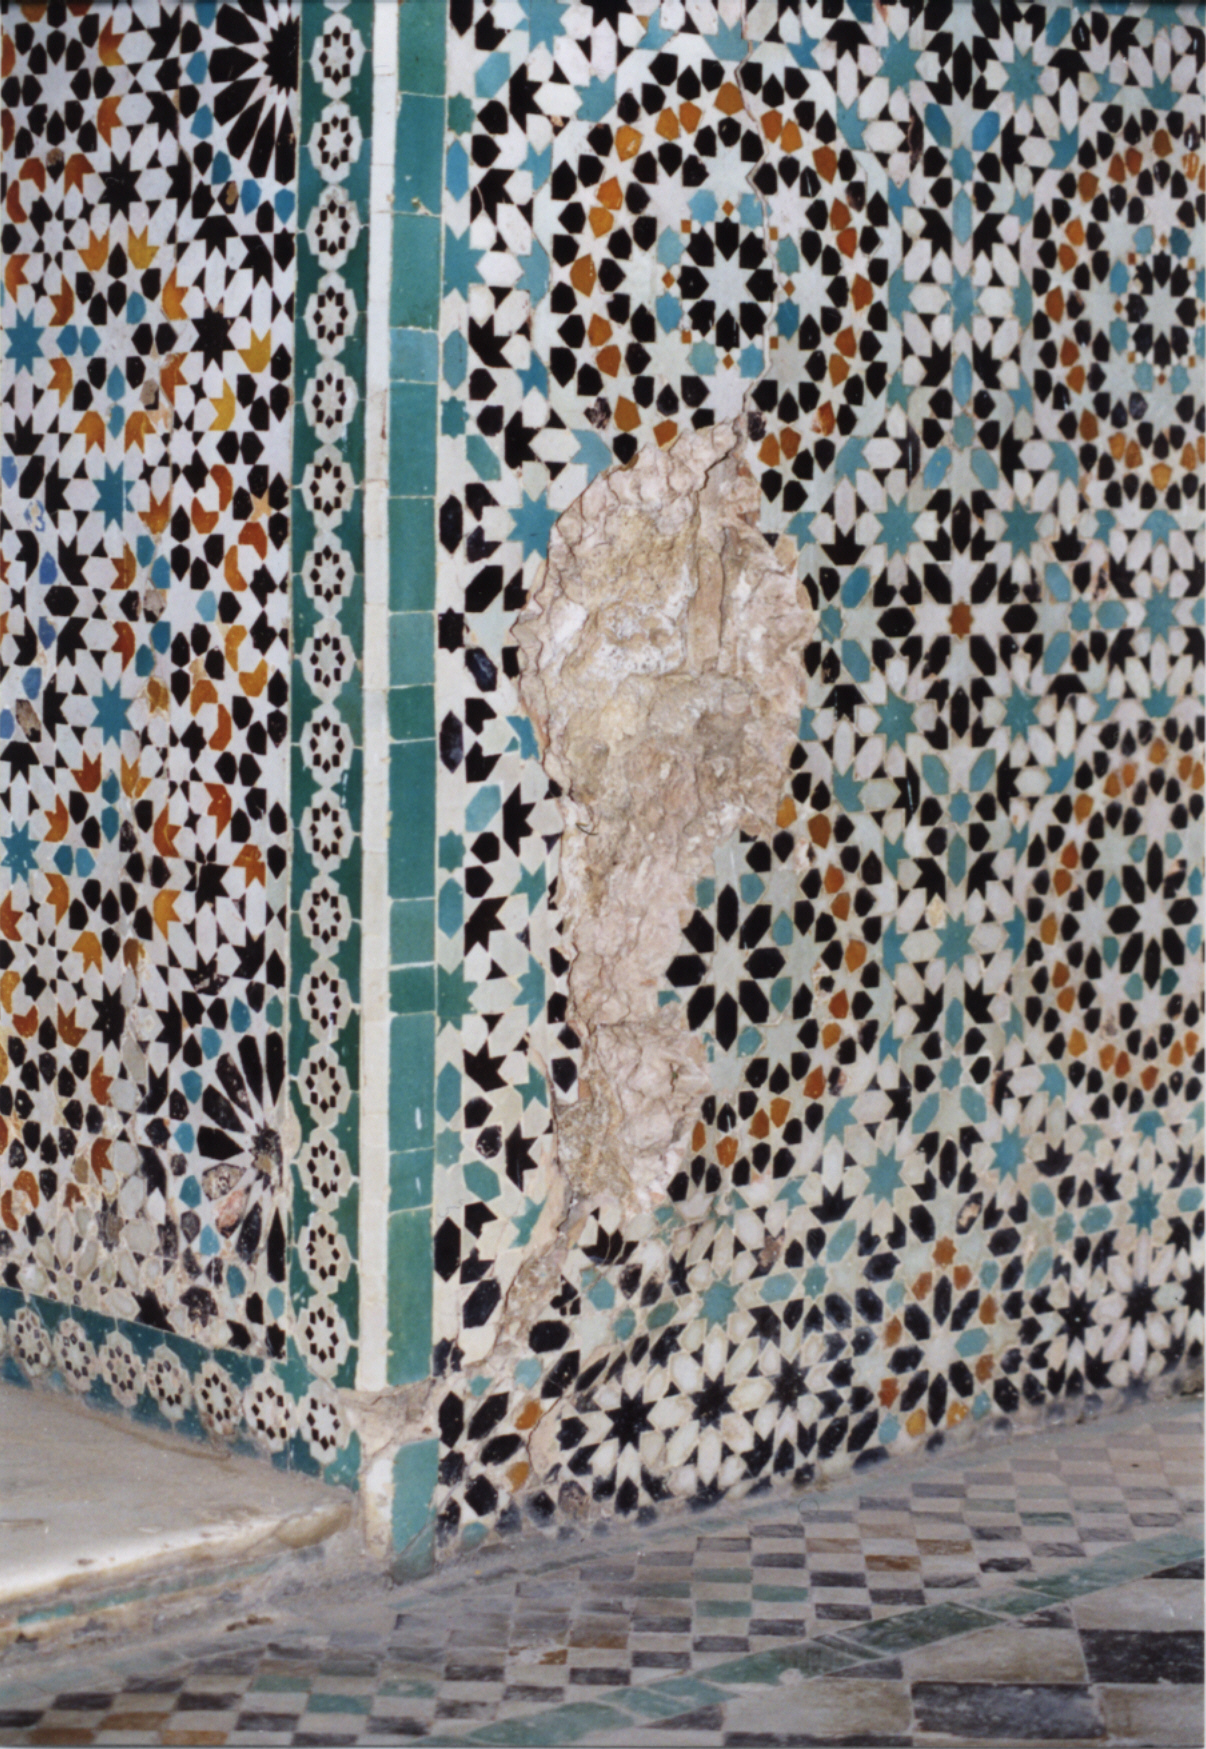
\includegraphics[width=0.45\textwidth]{alteration_1}%
%   \quad%
%   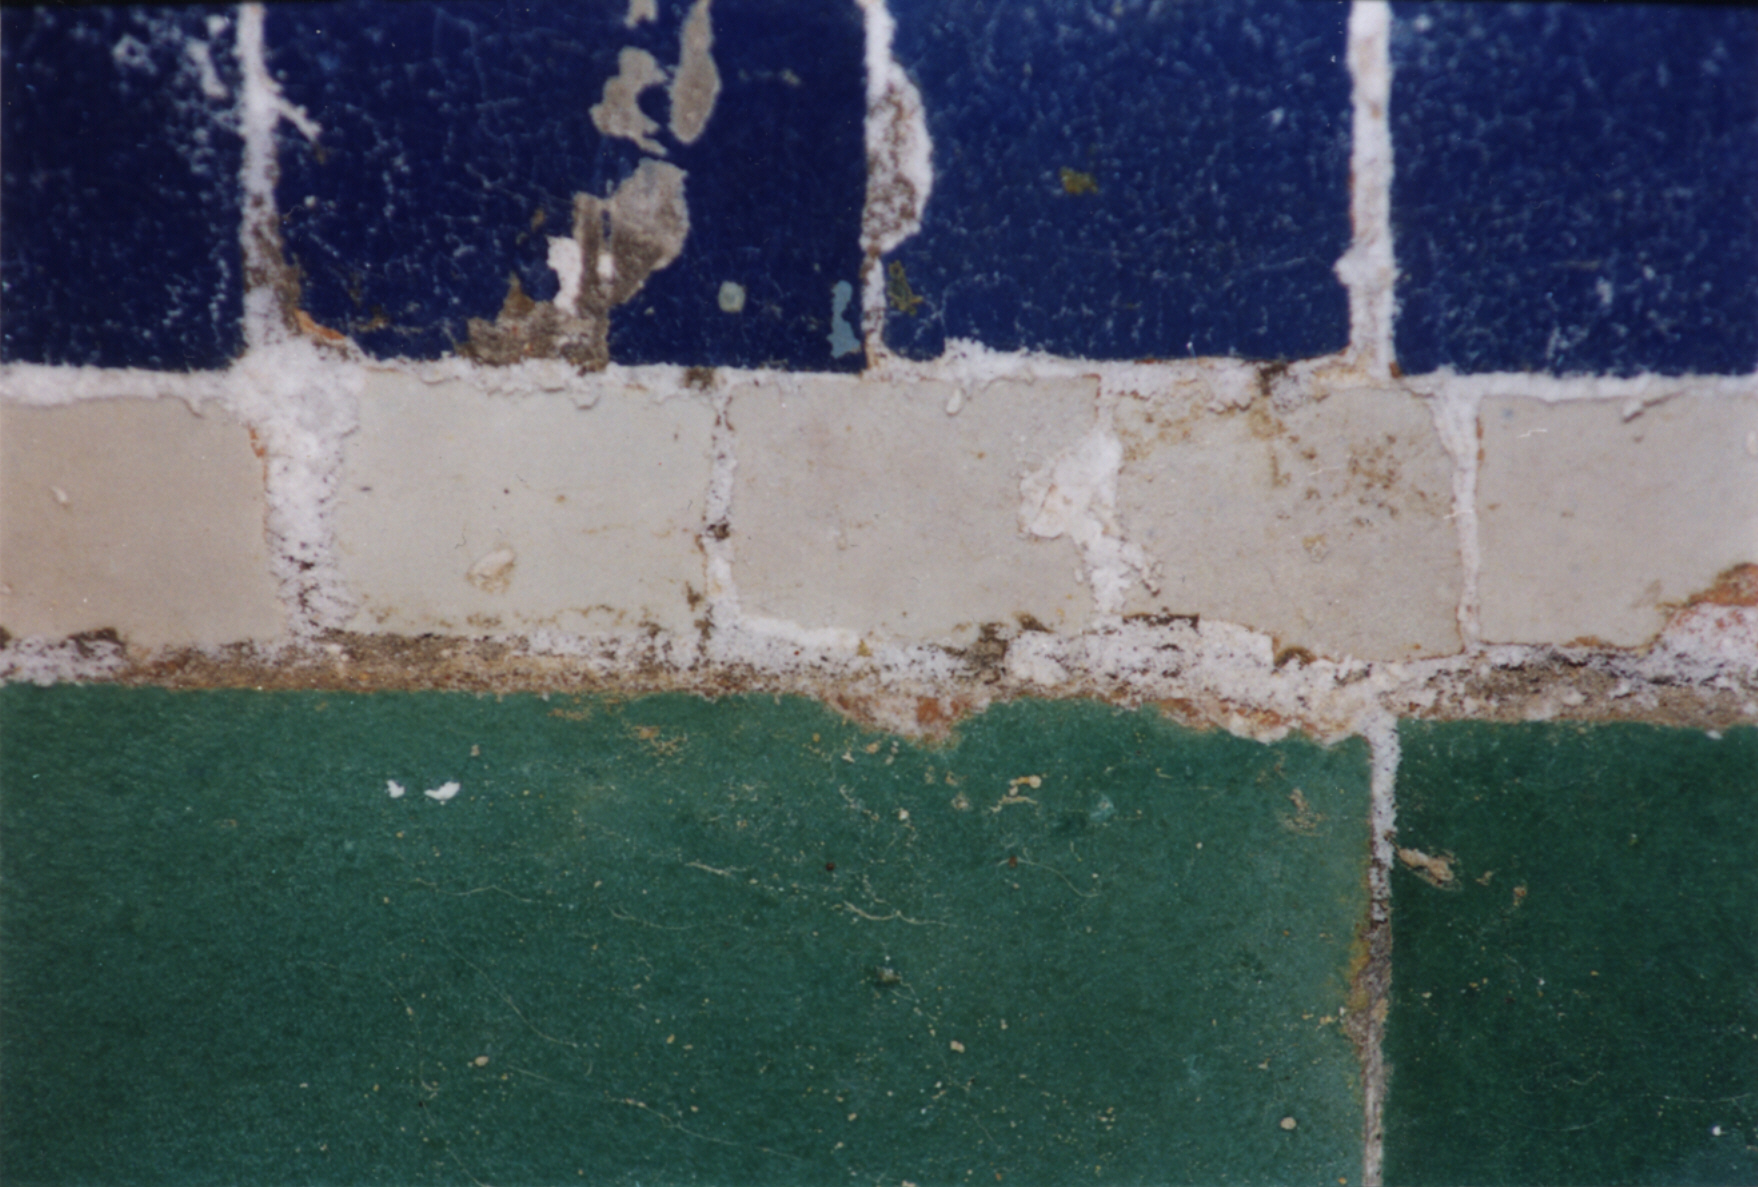
\includegraphics[width=0.45\textwidth]{alteration_2}
%   \caption{Différents types d'altération : à gauche, on note un 
%            décollement d'une partie du panneau décoré de zelliges ; 
%            à droite, des efflorescences salines sont visibles entre 
%            les pièces de céramique (clichés :~Schv{\oe}rer, 1999).}
%   \label{fig:alteration}
% \end{figure}

